\documentclass{article}

\usepackage{corl_2026} % CoRL 2026 initial submission (anonymized + line numbers + CoRL footer)

\usepackage{amsmath,amssymb,amsfonts}
\usepackage{graphicx}
\usepackage{subcaption}
\usepackage{url}

\title{Engineering Minimum-Cost Reach-Avoid Control for Quadruped Navigation}

\author{
  Anonymous Author(s)\\
  Affiliation\\
  Address\\
  \texttt{email}
}

\begin{document}
\maketitle

\begin{abstract}
This paper studies how to instantiate minimum-cost reach-avoid control on a real quadruped robot. Starting from RC-PPO, we identify the execution mismatch that appears when its idealized transition model is connected to a learned locomotion controller. To address this deployment gap, we construct a fixed and repeatable closed-loop velocity interface and calibrate execution-induced cost and trajectory errors into cost and safety margins. Simulation and physical-robot experiments evaluate each engineering module and the resulting navigation behavior.
\end{abstract}

\keywords{quadruped navigation, reach-avoid control, safe robot learning}

\section{Introduction}
Quadruped robots are increasingly used for inspection, exploration, and service
tasks in environments where a navigation policy must do more than reach a target.
The robot must remain collision-free during the whole maneuver while avoiding
unnecessary motion and energy expenditure. These requirements are coupled in
cluttered scenes: a short route may pass close to obstacles, whereas a safer route
may consume more time and actuation. Treating safety and efficiency as independent
reward terms therefore makes the desired trade-off dependent on hand-tuned weights.
Minimum-cost reach-avoid (MCRA) control provides a more direct task description by
requiring goal reachability and trajectory-wide avoidance while minimizing a
cumulative cost~\citep{bansal2017,ganai2024survey}.

Recent work has made MCRA learning practical through RC-PPO~\citep{so2024}.
RC-PPO augments the state with a safety indicator and remaining budget, learns a
reachability value function with a budget-conditioned policy, and then searches for
the least feasible initial budget. Together, these components provide a unified way
to represent safety and cost feasibility in the quadruped navigation task. However,
RC-PPO's reachability equivalence and budget-feasibility conclusions are established
under a nominal deterministic transition model. When connected to a real
quadruped, a high-level velocity command is not directly applied as a state
transition. Instead, it is realized through a locomotion controller, making the
physical closed-loop transition uncertain and dependent on contact conditions,
friction, actuation latency, and state-estimation error. Consequently, feasibility
under the nominal model does not automatically imply feasibility during physical
execution. This deployment mismatch appears as two task-relevant failures. First,
the executed path may be longer or slower, causing the nominal model to
underestimate cumulative cost. Second, the executed body path may deviate toward
an obstacle, causing a trajectory that is safe in the nominal map to lose clearance
on hardware.

This work focuses on instantiating RC-PPO/MCRA on a real quadruped by constructing
a fixed and repeatable closed-loop velocity interface and calibrating
execution-induced cost and trajectory errors. Following the failure modes above,
we train a locomotion tracker once and freeze it before high-level learning. This
interface reduces the navigation action space and, more importantly, defines a
repeatable closed-loop mapping whose residual error can be measured. We collect
paired nominal and executed rollouts through that mapping and use the resulting
error distributions to calibrate two separate corrections. A cost margin $\alpha$
inflates the running cost used by the budget update, while a safety margin
$\delta$ enlarges the unsafe set used by reach-avoid learning. We then apply the
budget-conditioned policy and two-phase search to this calibrated model.

Our engineering contribution is an execution-calibrated deployment pipeline that
connects an ideal MCRA learner to a physical closed loop. We do not claim a strict
stochastic safety guarantee or extend RC-PPO's deterministic theory to general
stochastic systems; instead, our claims are limited to empirical robustness under
the execution distribution used to calibrate the margins. We evaluate the pipeline
with controlled mismatch studies, component-wise ablations, sensitivity tests, and
a quantitative physical-robot deployment study. The experiments are designed to
answer where direct RC-PPO deployment fails, whether the frozen interface makes
the high-level problem repeatable, whether $\alpha$ and $\delta$ address different
failure modes, and how the complete system behaves on hardware.

Our contributions are:
\begin{enumerate}
\item We identify the model--execution mismatch that must be handled when an
      MCRA policy is deployed through a quadruped locomotion controller, separating
      cost overrun from geometric path deviation.
\item We develop an execution-calibrated deployment layer consisting of a frozen
      velocity interface, paired mismatch data, and two corrections that map
      measured cost and path errors to budget inflation ($\alpha$) and unsafe-set
      dilation ($\delta$).
\item We evaluate the resulting RC-PPO-based system through controlled studies and
      physical-robot trials, with the protocol and claim boundaries made explicit
      for each module.
\end{enumerate}

The remainder of the paper first positions HD-MCRA relative to MCRA learning,
quadruped navigation, and risk-aware planning. We then define the ideal MCRA
problem and its closed-loop deployment gap, describe the execution-calibrated
system, and evaluate each engineering choice before discussing limitations.

\section{Related Work}
\subsection{Minimum-Cost Reach-Avoid Learning}
Reach-avoid reinforcement learning treats reaching a target and avoiding an unsafe
set as trajectory-level requirements rather than competing reward terms
\citep{bansal2017,ganai2023}. RC-PPO extends this view to minimum-cost reach-avoid
control by augmenting the state with a safety indicator and remaining budget,
learning a budget-conditioned policy and reachability critic, and searching for the
least feasible initial budget~\citep{so2024}. This construction is the algorithmic
foundation used here. Our focus is the interface between its transition model and a
quadruped's executed motion, which is outside the deterministic model assumed by
the original formulation.

\subsection{Safe Quadruped Navigation}
Learning-based quadruped systems have demonstrated robust locomotion and navigation
over challenging terrain~\citep{hwangbo2019,lee2020,kumar2021,miki2022,hoeller2024}.
Recent navigation systems improve agility, perception or traversal in confined and
unstructured environments~\citep{miki2024,weerakoon2024,guerrier2024}. Safety is
also addressed through constrained policy optimization, control barrier functions,
and risk-sensitive objectives~\citep{achiam2017,liu2022cvpo,renganathan2023}.
These methods establish useful hardware interfaces and safety mechanisms, but they
do not directly provide the execution-data calibration procedure used here to
jointly adjust an MCRA budget and an avoid-set boundary.

\subsection{Robust Deployment under Model--Execution Mismatch}
Domain randomization and robust reinforcement learning address model uncertainty by
broadening the training distribution or optimizing for robustness across perturbed
dynamics~\citep{tobin2017,smirnova2019,wang2021,liu2022drql}. In contrast,
chance-constrained and risk-aware planners represent uncertainty at the planning
level through traversability, path-selection, or violation-risk models
~\citep{theurkauf2023,fan2021step,schmittle2024}. These approaches differ from the
present deployment layer in both object and mechanism. STEP estimates stochastic
traversability for risk-aware off-road planning, and Schmittle et al. use multiple
long-range samples under sensing uncertainty; HD-MCRA instead measures paired
nominal/executed errors after fixing a velocity interface, then maps upper empirical
quantiles to the MCRA running cost and unsafe set. The resulting claim is
correspondingly narrower: empirical robustness under the calibration distribution,
without a new formal stochastic guarantee.

The remaining gap is thus practical rather than theoretical: an MCRA learner needs
a repeatable closed-loop interface and an explicit procedure for converting its
measured execution mismatch into the two quantities that determine feasibility,
namely cumulative budget and geometric clearance.

\section{Problem Setup: From Ideal MCRA to Quadruped Execution}
\subsection{MCRA and RC-PPO Recap}
We model the navigation layer as a discrete-time process with state $x_t\in
\mathcal{X}$, high-level velocity command $u_t\in\mathcal{U}^{\mathrm{high}}$,
transition kernel $P$, running cost $c$, and initial-state distribution $\rho_0$.
The MCRA objective is to reach a goal set $\mathcal{G}$, avoid an unsafe set
$\mathcal{F}$ at every step, and minimize the accumulated cost until a free terminal
time $T$:
\begin{align}
\min_{\pi,T}\quad &\sum_{t=0}^{T-1}c(x_t,\pi(x_t))\\
\mathrm{s.t.}\quad &x_T\in\mathcal{G},\quad x_t\notin\mathcal{F}\ \forall t\leq T,
\quad x_{t+1}\sim P(\cdot\mid x_t,\pi(x_t)).
\end{align}
We represent the sets using signed functions $g$ and $h$ as
$\mathcal{G}=\{x:g(x)\leq0\}$ and $\mathcal{F}=\{x:h(x)>0\}$. Following
RC-PPO~\citep{so2024}, the state is augmented to $\hat{x}_t=(x_t,y_t,z_t)$,
where $y_t\in\{-1,1\}$ records whether the unsafe set has been entered and $z_t$
is remaining budget. The shifted indicator is
$I_{b\in\mathcal{B}}=+1$ when $b\in\mathcal{B}$ and $-1$ otherwise; thus
$y_{t+1}=\max\{I_{x_{t+1}\in\mathcal{F}},y_t\}$ and
$z_{t+1}=z_t-c(x_t,u_t)$. The augmented goal function is
\begin{equation}
\hat{g}(x,y,z)=\max\{g(x),Cy,-z\},
\end{equation}
where $C>0$ is an arbitrary safety-violation constant. RC-PPO notes that a
practical choice is $C=\max_{x\in\mathcal{X}}g(x)$~\citep{so2024}. Reaching the
zero sublevel set of $\hat{g}$ therefore encodes goal reaching, trajectory-wide
avoidance, and the upper-bound property $z_0\geq\sum_t c_t$. Following RC-PPO, we
use its reachability critic, budget-conditioned actor, and two-phase minimum-budget
search as the high-level decision backbone. The remainder of this section defines
how that backbone is connected to the quadruped's closed-loop execution and where
the resulting model--execution mismatch enters the deployment problem.

\subsection{Quadruped Closed-Loop Execution}
On hardware, $u_t$ is a desired body velocity that is realized by a locomotion
controller. Let $P_{\mathrm{cl}}$ denote the induced closed-loop transition after
this controller is applied. The nominal model used by high-level learning is
$x_{t+1}=\bar f_{\mathrm{cl}}(x_t,u_t)$, while the executed transition is sampled
from $P_{\mathrm{cl}}(\cdot\mid x_t,u_t)$. The difference is the deployment gap
addressed by HD-MCRA. For a paired nominal/executed rollout, we define the relative
cost overrun and a trajectory-deviation statistic as
\begin{equation}
\varepsilon_c=\frac{J_{\mathrm{exec}}-J_{\mathrm{nom}}}{J_{\mathrm{nom}}},
\qquad
\varepsilon_d=d(\tau_{\mathrm{exec}},\tau_{\mathrm{nom}}),
\end{equation}
where the exact cost units, trajectory distance, time window, and pairing protocol
are specified with the experiment data. These implementation-level quantities are
currently marked \textsc{TBD} pending the original configuration and logs.

\subsection{Deployment Objective and Scope}
The deployment objective is to retain the RC-PPO MCRA semantics while accounting
for the measured distribution of $(\varepsilon_c,\varepsilon_d)$. HD-MCRA treats
these quantities as empirical descriptions of the nominal-to-execution gap rather
than as a new stochastic reachability model. The next section describes how a
fixed velocity interface, paired rollout data, and calibrated margins are used to
make this gap actionable for high-level learning and deployment.

\section{Execution-Calibrated HD-MCRA}
% TASK-010--TASK-012: interface, mismatch dataset, alpha/delta calibration,
% robustified RC-PPO learning and deployment algorithm.
\subsection{System Overview}
Figure~\ref{fig:system_overview} summarizes the deployment pipeline. The problem
setup in Section~3 defines the nominal-to-execution errors, while this section
specifies how they are measured and used. Components inherited from RC-PPO are
kept fixed, and the execution calibration layer is fitted before high-level policy
training. Offline rollouts produce paired nominal and executed trajectories; their
cost and geometric errors are converted into $\alpha$ and $\delta$. The corrected
model is then used for high-level learning and budget search. Online, the policy
emits a velocity command and the frozen tracker closes the loop on the robot.

\begin{figure}[t]
\centering
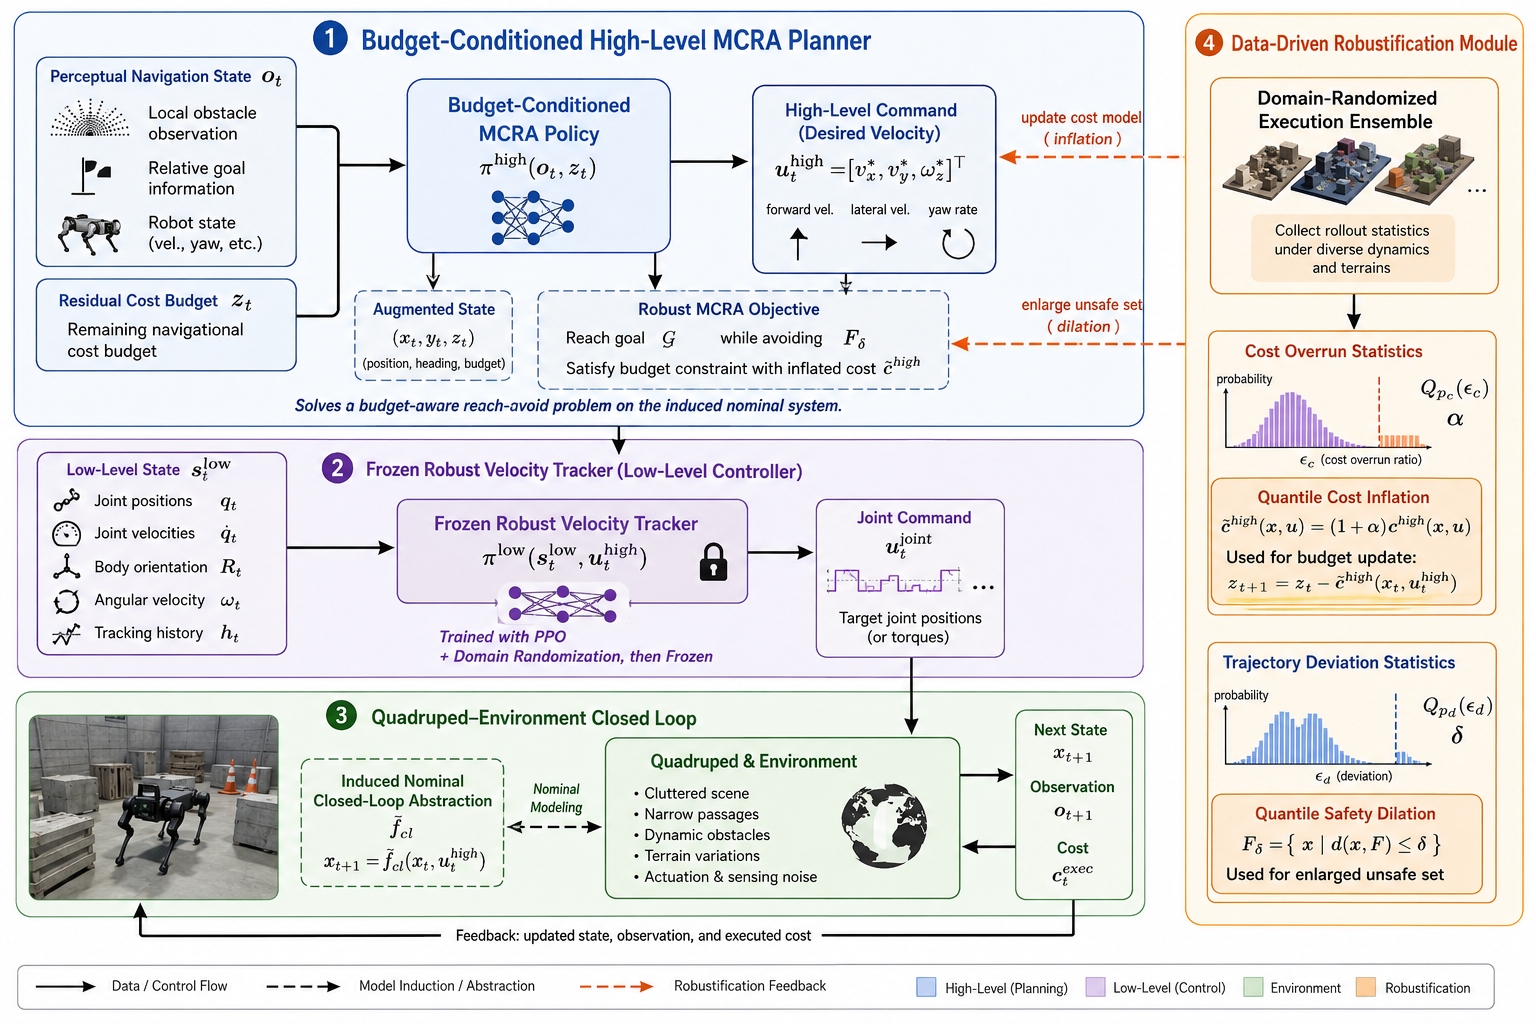
\includegraphics[width=0.96\columnwidth]{../../images/framework_overview_final.png}
\caption{HD-MCRA deployment pipeline. The frozen velocity tracker supplies the
execution interface; the calibration stage maps paired nominal/executed rollouts
to the cost margin $\alpha$ and safety margin $\delta$.}
\label{fig:system_overview}
\end{figure}

\subsection{Frozen Velocity-Control Interface}
To make the nominal-to-execution gap measurable through a consistent execution
interface, we first establish a fixed closed-loop velocity interface between the
high-level navigation policy and the quadruped. The low-level controller maps
proprioceptive observations and body-velocity commands
$u_t=[v_x^*,v_y^*,\omega_z^*]^\top$ to joint commands. It is pretrained using PPO
and domain randomization, then frozen before execution-mismatch calibration and
high-level learning. Freezing keeps the controller parameters unchanged, avoiding
interface changes caused by continued low-level policy updates. It does not make
the physical closed loop deterministic: contact conditions, friction, actuation
latency, and state-estimation error can still produce residual mismatch.

We obtain the nominal closed-loop map $\bar f_{\rm cl}$ by rolling out the frozen
tracker under nominal dynamics and recording the state at the high-level decision
interval. The same tracker and command domain are used for calibration, high-level
learning, and deployment, so the measured errors refer to the interface used by the
navigation policy. Tracking accuracy and locomotion stability must be verified
within this domain. The next subsection describes how paired nominal and executed
rollouts measure the remaining cost and trajectory errors. Specific command limits
and training configurations are listed in Appendix~\ref{app:velocity_interface}.

\subsection{Execution-Mismatch Dataset}
We construct a calibration set by replaying the same high-level command sequences
through the nominal closed-loop model and through perturbed executions. Each pair
shares the initial state, map, goal, and command sequence. This operationalizes the
abstract mismatch variables defined in Section~3. For a rollout of length $T$, let
$J_{\rm nom}=\sum_{t=0}^{T-1}c(x_t^{\rm nom},u_t)$ and
$J_{\rm exec}=\sum_{t=0}^{T-1}c(x_t^{\rm exec},u_t)$. The draft uses 1,200 paired
rollouts, with 800 for calibration and 400 held out for evaluation~\textit{(assumed
data)}. Perturbations cover friction, actuation delay and velocity-tracking noise;
LiDAR perturbations are evaluated separately because they affect the policy's
observation rather than the same-command execution mismatch. Exact perturbation
ranges and their assignment to calibration or held-out conditions remain
\textsc{TBD}.

The relative cost overrun $\varepsilon_c$ is computed from the paired cumulative
costs. For geometric deviation, the draft uses the maximum planar distance between
time-aligned body poses,
\begin{equation}
\varepsilon_d=\max_{0\leq t\leq T} \left\|p_t^{\rm exec}-p_t^{\rm nom}\right\|_2,
\end{equation}
where $p_t$ is the base position. Samples are split by rollout before quantile
estimation to avoid leakage. These definitions and sample counts are placeholders
for the real data and are explicitly marked as assumed.

\subsection{Cost and Safety Calibration}
The two error channels are calibrated independently because they affect different
MCRA constraints. For calibration quantiles $p_c$ and $p_d$, we set
\begin{equation}
\alpha=Q_{p_c}(\varepsilon_c),\qquad
\delta=Q_{p_d}(\varepsilon_d),
\end{equation}
with $p_c=p_d=0.90$ in the draft~\textit{(assumed data)}. The resulting values are
$\alpha=0.18$~\textit{(assumed data)} and $\delta=0.12$ m~\textit{(assumed data)}.
The calibrated running cost is
$\tilde c(x_t,u_t)=(1+\alpha)c(x_t,u_t)$, so the remaining budget evolves as
$z_{t+1}=z_t-\tilde c(x_t,u_t)$. The safety correction dilates the unsafe set by
$\mathcal{F}_\delta=\{x:d(x,\mathcal{F})\leq\delta\}$. If the robot footprint is
already included in the map obstacle layer, $\delta$ is an additional execution
margin rather than a second footprint inflation; this implementation detail is
\textsc{TBD}.

This empirical coverage interpretation is limited to the calibration distribution;
it does not provide a formal stochastic safety guarantee under arbitrary
execution shifts. The next subsection describes how the calibrated cost and unsafe
set are incorporated into the inherited RC-PPO learning and budget-search procedure.

\subsection{Robust MCRA Learning and Deployment}
With $\tilde c$ and $\mathcal{F}_\delta$, the high-level learner follows the
RC-PPO two-phase procedure. In Phase I, a stochastic actor
$\pi_\theta(u\mid o,z)$ and reachability critic $V_\psi(\hat x)$ are optimized on
the augmented state. The PPO ratio objective is
\begin{equation}
L^{\rm clip}(\theta)=\mathbb{E}_t\left[\min\left(r_t(\theta)\hat A_t,
\operatorname{clip}(r_t(\theta),1-\epsilon,1+\epsilon)\hat A_t\right)\right],
\end{equation}
where $r_t(\theta)=\pi_\theta(u_t\mid o_t,z_t)/\pi_{\theta_{\rm old}}(u_t\mid
o_t,z_t)$. The advantage uses the reachability critic and generalized advantage
estimation; $\epsilon$ is the PPO clipping parameter. The critic target is the
discounted reachability Bellman target with the augmented goal function, evaluated
using the nominal closed-loop transition and the corrected budget/unsafe-set
definitions. At a goal, collision, budget violation or time-limit terminal, the
bootstrap term is set to zero; this terminal handling is stated explicitly because
it was absent from the 0820 description.

The draft samples $z_0/z_{\rm ref}$ uniformly from $[0.8,1.2]$ during Phase I and
uses $\gamma=0.99$, $\epsilon=0.2$ and GAE $\lambda=0.95$~\textit{(assumed data)}.
These values are placeholders. In Phase II, the stochastic actor is replaced by
its mean action. The least feasible budget is found by scanning the normalized grid
$\{0.80,0.85,0.90,0.96,1.00,1.05,1.12,1.20\}$~\textit{(assumed data)} and
selecting the smallest value meeting the stated success, collision and budget
criteria. This search is inherited from RC-PPO; the engineering change is that the
search uses the calibrated closed-loop model.

For the assumed-data draft, confidence intervals are intentionally omitted rather
than reconstructed from aggregate means or plotted bars. The final protocol should
report binomial intervals for SR/CR/BVR, bootstrap intervals for cost and MC, and
the quantile estimation uncertainty for $\alpha$ and $\delta$, all computed from
the original trial-level records.

\paragraph{Execution-calibrated procedure.}
The draft implementation follows five steps:
\begin{enumerate}
\item Freeze the velocity tracker and collect paired nominal/executed rollouts.
\item Estimate $\alpha$ and $\delta$ from held-out calibration quantiles.
\item Train the budget-conditioned RC-PPO actor and critic using $\tilde c$ and
      $\mathcal{F}_\delta$.
\item Convert the actor to mean-action deployment and search the feasible budget
      grid.
\item Execute the selected policy and log goal, safety and cost outcomes.
\end{enumerate}

\section{Experiments}
% TASK-013--TASK-014: RQ1--RQ5 protocol, results and analysis.
\subsection{Experimental Protocol}
We organize the evaluation around five questions. RQ1 measures the direct
nominal-to-executed gap. RQ2 tests whether the frozen interface makes the
high-level transition sufficiently repeatable. RQ3 isolates the roles of $\alpha$
and $\delta$. RQ4 studies sensitivity to the margins and to execution conditions
outside calibration. RQ5 evaluates the full pipeline on a Unitree Go2.

The draft protocol uses a simulated differential-drive abstraction coupled to the
same velocity interface and three map families: moderately cluttered, narrow
passage and densely obstructed. Each method receives the same local LiDAR scan,
relative goal and robot state. The high-level decision interval is 0.2 s and the
episode horizon is 30 s~\textit{(assumed data)}. We report success rate (SR),
collision rate (CR), cumulative cost, budget violation rate (BVR), and minimum
clearance (MC). A trial is successful only if it reaches the goal before the time
limit without entering the unsafe set; a budget violation is recorded when the
executed cumulative cost exceeds the selected initial budget. The exact simulator
version and random-seed count are \textsc{TBD}; the draft uses 3 seeds and 300
trials per method~\textit{(assumed data)}.

For fair comparison, RC-PPO uses the same frozen velocity interface and training
budget as HD-MCRA but sets $\alpha=0$ and $\delta=0$. RA denotes reach-avoid
learning without cost conditioning. PPO$_{\beta_L}$ and PPO$_{\beta_H}$ are
reward-shaped policies with low and high safety weights; CPPO variants use the same
weights in a constrained objective. These baseline implementations are provisional
and must be checked against the original configuration.

\subsection{RQ1: Direct Deployment Gap}
The first experiment compares nominal and executed rollouts before any margin is
applied. Under the draft perturbation distribution, the median relative cost
overrun is $0.09$~\textit{(assumed data)} and the 90th percentile is
$0.18$~\textit{(assumed data)}. The corresponding maximum path deviation has a
median of $0.06$ m and a 90th percentile of $0.12$ m~\textit{(assumed data)}.
These values motivate the draft settings $\alpha=0.18$ and $\delta=0.12$ m; they
are not claims about the final robot logs. Direct RC-PPO evaluated without these
corrections yields an assumed BVR of $14.0\%$ and CR of $15.7\%$ across the three
maps~\textit{(assumed data)}, illustrating why nominal feasibility is insufficient.

\subsection{RQ2: Closed-Loop Interface}
To isolate hierarchy, we compare the frozen velocity interface with a joint-space
variant that exposes the high-level learner to 12 actuator targets. The joint-space
variant uses the same PPO optimizer and training steps. In the draft, the frozen
interface reduces the command-tracking RMSE from $0.19$ to $0.08$ (velocity units)
and increases converged training runs from $7/10$ to $9/10$~\textit{(assumed data)}.
The comparison is intended to test stationarity and controllability, not to claim a
new low-level controller.

\subsection{RQ3: Cost and Safety Margins}
Table~\ref{tab:main_results} reports the draft comparison. Every number in this
table is an assumed placeholder for structural review and must be replaced by
trial-level measurements. The full system improves the cost-feasibility metric
relative to uncalibrated RC-PPO while retaining a similar collision rate.

\begin{figure}[t]
\centering
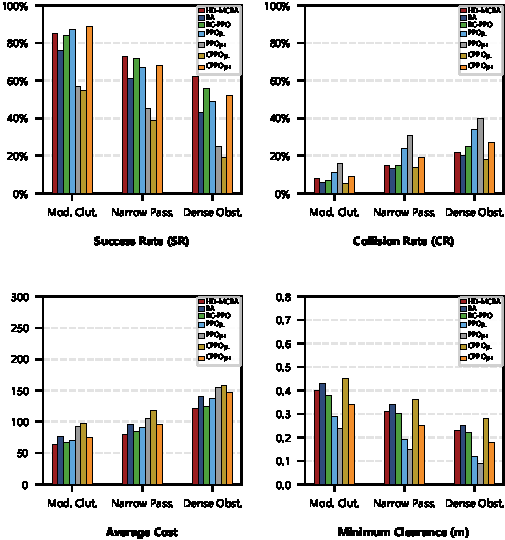
\includegraphics[width=\columnwidth]{../../images/figure_metrics_grid_single_column_v3.pdf}
\caption{Draft scenario-level performance trends. All plotted values are assumed
data placeholders and must be regenerated from trial logs.}
\label{fig:metrics_draft}
\end{figure}

\begin{table}[t]
\caption{Draft average performance over three simulated scenarios (all entries are assumed data).}
\label{tab:main_results}
\centering
\resizebox{\columnwidth}{!}{%
\begin{tabular}{lccccc}
\hline
Method & SR (\%) & CR (\%) & Cost & BVR (\%) & MC (m)\\
\hline
HD-MCRA & 73.3~\textit{(assumed data)} & 15.0~\textit{(assumed data)} & 88.3~\textit{(assumed data)} & 9.0~\textit{(assumed data)} & 0.31~\textit{(assumed data)}\\
RC-PPO & 70.7~\textit{(assumed data)} & 15.7~\textit{(assumed data)} & 91.7~\textit{(assumed data)} & 14.0~\textit{(assumed data)} & 0.30~\textit{(assumed data)}\\
RA & 60.0~\textit{(assumed data)} & 13.0~\textit{(assumed data)} & 104.0~\textit{(assumed data)} & 22.0~\textit{(assumed data)} & 0.34~\textit{(assumed data)}\\
PPO$_{\beta_L}$ & 67.7~\textit{(assumed data)} & 23.0~\textit{(assumed data)} & 99.7~\textit{(assumed data)} & 20.7~\textit{(assumed data)} & 0.20~\textit{(assumed data)}\\
PPO$_{\beta_H}$ & 42.3~\textit{(assumed data)} & 29.0~\textit{(assumed data)} & 117.0~\textit{(assumed data)} & 27.0~\textit{(assumed data)} & 0.16~\textit{(assumed data)}\\
CPPO$_{\beta_L}$ & 37.7~\textit{(assumed data)} & 12.3~\textit{(assumed data)} & 124.7~\textit{(assumed data)} & 22.3~\textit{(assumed data)} & 0.36~\textit{(assumed data)}\\
CPPO$_{\beta_H}$ & 69.7~\textit{(assumed data)} & 18.3~\textit{(assumed data)} & 105.7~\textit{(assumed data)} & 17.0~\textit{(assumed data)} & 0.26~\textit{(assumed data)}\\
\hline
\end{tabular}}
\end{table}

The component-wise ablation in Table~\ref{tab:ablation_draft} follows the same
evaluation batch. Removing $\alpha$ primarily increases BVR, whereas removing
$\delta$ reduces clearance and increases CR. Removing the hierarchy has the
largest combined degradation. These are intended causal patterns; the assumed
values must be replaced together with confidence intervals.

\begin{table}[t]
\caption{Draft component ablation (all entries are assumed data).}
\label{tab:ablation_draft}
\centering
\resizebox{\columnwidth}{!}{%
\begin{tabular}{lccccc}
\hline
Variant & SR (\%) & CR (\%) & Cost & BVR (\%) & MC (m)\\
\hline
w/o hierarchy & 47.9~\textit{(assumed data)} & 38.8~\textit{(assumed data)} & 116.7~\textit{(assumed data)} & 31.5~\textit{(assumed data)} & 0.11~\textit{(assumed data)}\\
w/o $\alpha$ & 67.2~\textit{(assumed data)} & 19.8~\textit{(assumed data)} & 80.6~\textit{(assumed data)} & 22.4~\textit{(assumed data)} & 0.29~\textit{(assumed data)}\\
w/o $\delta$ & 64.8~\textit{(assumed data)} & 26.3~\textit{(assumed data)} & 77.2~\textit{(assumed data)} & 13.8~\textit{(assumed data)} & 0.19~\textit{(assumed data)}\\
w/o both & 62.9~\textit{(assumed data)} & 29.4~\textit{(assumed data)} & 87.6~\textit{(assumed data)} & 25.8~\textit{(assumed data)} & 0.16~\textit{(assumed data)}\\
HD-MCRA & 70.8~\textit{(assumed data)} & 18.6~\textit{(assumed data)} & 71.3~\textit{(assumed data)} & 11.2~\textit{(assumed data)} & 0.32~\textit{(assumed data)}\\
\hline
\end{tabular}}
\end{table}

\subsection{RQ4: Sensitivity and Distribution Shift}
We sweep $\alpha\in\{0,0.09,0.18,0.27\}$ and
$\delta\in\{0,0.06,0.12,0.18\}$ m~\textit{(assumed data)}. The draft trend is
monotonic reduction of BVR with increasing $\alpha$ and monotonic reduction of CR
with increasing $\delta$, accompanied by higher path cost and occasional lower SR
when margins become excessive. Under a held-out perturbation level 25\% larger than
calibration, the assumed full system retains SR $65.0\%$ and BVR $16.0\%$,
whereas the uncalibrated baseline reaches SR $58.0\%$ and BVR $24.0\%$~\textit{(assumed
data)}. These values illustrate the intended stress test but do not establish a
distribution-free guarantee.

\begin{figure}[t]
\centering
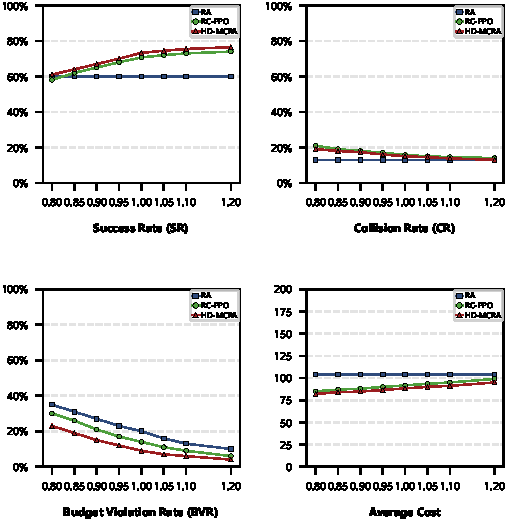
\includegraphics[width=\columnwidth]{../../images/figure_budget_sweep_v3.pdf}
\caption{Draft budget-response curves. Curves are assumed data placeholders for
protocol review.}
\label{fig:budget_draft}
\end{figure}

\subsection{RQ5: Physical-Robot Deployment}
The draft physical study uses a Unitree Go2 in a cluttered indoor environment with
chairs, narrow passages and a moving obstacle. The representative route length is
approximately 15 m and the narrow passage is about 0.3 m wider than the robot
body~\textit{(assumed data, inherited from the 0820 description)}. The assumed
deployment count is 26 successful trials out of 30, corresponding to SR $86.7\%$
~\textit{(assumed data)}. The remaining four trials are provisionally classified as
two localization failures, one conservative timeout and one contact with a chair
leg~\textit{(assumed data)}. This classification must be replaced by the actual
trial log. We report the deployment as an engineering study, not as a statistical
certification.

\section{Limitations}
The current manuscript is an engineering draft and has several limitations. First,
the numerical values in this version are explicitly assumed placeholders; no result
should be used for a scientific comparison until replaced by trial-level logs and
confidence intervals. Second, the robustness mechanism uses fixed empirical
quantiles and therefore only describes coverage under the calibration distribution.
Temporal correlation, rare contacts and distribution shifts can make the effective
coverage lower than the marginal quantile suggests. Third, a fixed $\alpha$ may be
overly conservative in open space and insufficient under severe actuator or
perception faults, while a fixed $\delta$ can remove feasible narrow passages.
Fourth, the LiDAR observation can miss thin structures or obstacles behind
occlusions. Finally, the current physical study is small and indoor; broader
terrain, payload and weather conditions are required before making claims about
general quadruped deployment.

\section{Conclusion}
This paper reframes the practical use of RC-PPO/MCRA on a quadruped as a deployment
problem. The MCRA objective, augmented state and two-phase solver are inherited
from prior work. The new engineering layer fixes a velocity-level closed-loop
interface, measures paired nominal/executed mismatch, and maps cost overrun and
path deviation to separate corrections $\alpha$ and $\delta$. This organization
turns an abstract budget-conditioned reach-avoid learner into a pipeline that can
be calibrated, tested and deployed on a physical robot. The present numerical
results are placeholders marked as assumed data; the final conclusions will be
updated after replacing them with verified simulation and Go2 logs. The intended
claim is empirical robustness within the calibrated execution distribution, not a
new formal stochastic reach-avoid guarantee.

\clearpage
\appendix
\section{Velocity-Interface Implementation Details}
\label{app:velocity_interface}
The draft command limits for the frozen velocity tracker are
$v_x^*\in[-0.6,0.6]$ m/s, $v_y^*\in[-0.4,0.4]$ m/s, and
$\omega_z^*\in[-1.2,1.2]$ rad/s~\textit{(assumed data)}. These values are
provisional configuration placeholders and must be verified against the original
implementation before submission.

The exact network architecture, reward weights, domain-randomization ranges, and
low-level and high-level control rates remain \textsc{TBD} pending restoration of
the original configuration. Tracking accuracy and locomotion stability must be
reported over the command domain used for calibration, learning, and deployment.

\bibliography{references}

\end{document}
